\documentclass[11pt]{scrartcl}
\usepackage{graphicx}
\graphicspath{{./}}
\usepackage[sexy]{evan}
\usepackage[normalem]{ulem}
\usepackage{hyperref}
\usepackage{mathtools}
\hypersetup{
    colorlinks=true,
    linkcolor=blue,
    filecolor=magenta,      
    urlcolor=cyan,
    pdfpagemode=FullScreen,
    }

\renewcommand{\baselinestretch}{1.5}

\addtolength{\oddsidemargin}{-0.4in}
\addtolength{\evensidemargin}{-0.4in}
\addtolength{\textwidth}{0.8in}

\setlength{\parindent}{0pt}

\usepackage{pgfplots}
\pgfplotsset{compat=1.15}
\usepackage{mathrsfs}
\usetikzlibrary{arrows}

\begin{document}
	\title{Daily Problems Set} % Beginner
	\date{}
	\author{Mini 1}
	\maketitle

	\section{Soal}
	\begin{enumerate}
	    \item Pada $\triangle ABC$ terdapat titik $D$ pada segmen $BC$ sehingga $BD:DC=1:3$. Titik $L$ pada $AD$ sehingga $AL:LD=1:4$. Jika $\dfrac{[ACL]}{[BDL]}=k$, tentukan nilai $200k$.
            \begin{center}
                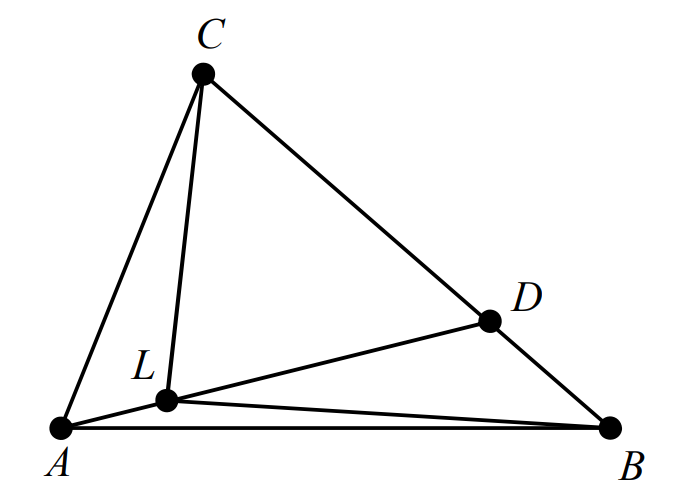
\includegraphics[scale=0.5]{geogampang.PNG}
            \end{center}
	    
	    
	    \item Misalkan suatu fungsi $f:\RR \rightarrow \RR$ memenuhi $f(xy)=f(x+y)$ untuk seluruh bilangan real $x$ dan $y$. Jika $f(-10)=10$ berapakah nilai $2021\cdot f(2021)$?
	    
	    \item Banyaknya pasangan terurut bilangan asli $(m,n)$ yang memenuhi $$m^3+n^3=(m+n)^2$$ adalah \dots    
	    
	    \item Berapa banyak bilangan bulat positif 8 digit yang memenuhi perkalian dari digit-digitnya adalah $2^{21}$?
	\end{enumerate}
	
\end{document}